% !TEX root = ms.tex
\chapter{Introducción}

La palabra \emph{"inteligencia artificial"} ha sido seleccionada por el
diccionario Collins como palabra del año en el 2023. Miles de empresas ahora
estan integrando tecnologías con \emph{"IA"}. Del mismo modo, multiples medios
de comunicación informan de los posibles problemas y riesgos de estas
tecnologías en caso de no ser implementadas de forma apropiada. A pesar de su
creciente popularidad en los ultimos años, el concepto de inteligencia
artificial es dificil de definir y categorizar incluso dentro del sector
cientifico.

Dado este contexto de creciente interés y debate, el presente capítulo
abordará los fundamentos de la inteligencia artificial, definiendo
sus características principales, su historia y las razones detrás de su
surgimiento.  Este marco conceptual es clave para que el lector pueda comprender
el estado del arte, que será tratado en profundidad en los capítulos siguientes.

\section{Inteligencia Artificial}
Las dos palabras acuñadas en el concepto de Inteligencia Artificial hacen
referencia a la simbiosis de dos campos de estudio totalmente diferentes. Es
tanto así, que en distintos idiomas esta composición lingüistica se mantiene
constante (véase la terminología en ingles: \emph{"Artificial Intelligence"}).

En este sentido, la \emph{inteligencia} ha sido estudiada historicamente por
ramas como la psicología, filosofía o educación donde se converge en multiples
definiciónes que aunque distintas, resultan "intuitivamente" faciles de
relacionar: la inteligencia hara referencia a la capacidad para entender,
comprender o resolver problemas, al conjunto de habilidades cognitivas que
incluyen la autoconciencia, creatividad o razonamiento logico. Fuera del ámbito
cientifico resulta sencillo distinguir aquellas entidades que demuestran
inteligencia de aquellas que no. Así pues, aunque puede conformarse un debate en
torno a las capacidades intelectuales de dos especies de similar origen (como lo
podría ser un delfín y un tiburon); es posible afirmar con certeza que una
unidad morfológica simple como lo es una celula eucariota, es menos inteligente
que un humano promedio.

De forma similar, todo aquello que es \emph{artificial} hace referencia a
aquello que no es natural, generalmente en relación con artefactos o productos
creados con un proposito determinado. Mientras que un delfín se puede considerar
producto de la naturaleza, un robot aspirador se considera artificial al ver que
este es consecuencia de una composición de elementos electronicos diseñados y
organizados por el ser humano con un fin concreto: limpiar el escenario en el
que se encuentre.

\begin{figure}[t]
    \centering
    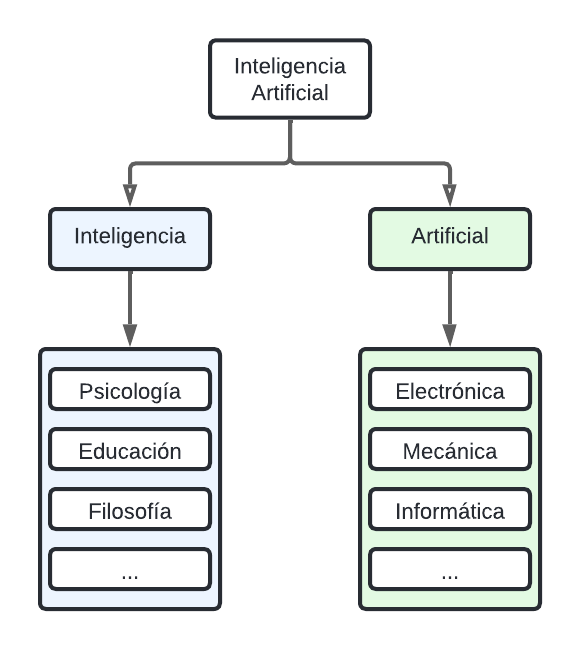
\includegraphics[scale=0.8, trim=0.5cm 0.5cm 0.5cm 0.5cm]{figs/artificial-vs-intelligence.png}
    \caption{\small"Inteligente" vs "Artificial". Elaboración Propia}
    \label{fig:etiqueta}
\end{figure}

Tras la Conferencia de Dartmouth organizada en 1956 por el matemático John McCarthy
junto con otro investigadores como Marvin Misnky, se definieron por primera vez las
bases de la inteligencia artificial:

\begin{quote}
    \textit{
        "El estudio procederá sobre la base de la conjetura de que cada aspecto
        del aprendizaje o cualquier otra característica de la inteligencia
        puede, en principio, ser descrito con tal precisión que se pueda crear
        una máquina capaz de simularlo." \citet{mccarthy2006proposal}
    }
\end{quote}

A lo largo de las decadas posteriores, el concepto de inteligencia artificial (IA) podrá
definirse entorno a 3 interpretaciónes de distintos sectores:

\begin{itemize}
    \item Desde la perspectiva de la IA clásica, desarrollada principalmente por
    los campos de las matemáticas e informática, la inteligencia artificial se
    concibe como un conjunto de algoritmos predefinidos, reglas de inferencia y
    razonamientos lógicos que buscan tomar decisiones, realizar tareas complejas
    o resolver problemas de manera autónoma. El objetivo de la IA clásica es
    resolver tareas como encontrar el camino más corto entre dos puntos o
    seleccionar el movimiento con mayor probabilidad de éxito en un juego como
    el ajedrez. 

    \item Desde la perspectiva del aprendizaje automático, la inteligencia
    artificial se define como una propiedad emergente de modelos matemáticos
    complejos, cuya interpretación no se basa en una secuencia de pasos
    predeterminada sino en las interacciones del modelo como conjunto. En este
    caso, de forma similar a como un cuadro artistico emerge como consecuencia
    del agrupamiento de trazos y colores adecuadamente posicionados, la IA
    emergera como resultado de las interacciones entre diferentes entidades
    matemáticas.  \footnote{Cabe señalar que, bajo este enfoque, la IA no puede
    ser controlada de forma determinista, ya que los modelos matemáticos no
    definen en su totalidad el comportamiento resultante de su aplicación.}

    \item Desde la perspectiva del campo de la cognición (interpretación que
    utilizada de aquí en adelante en esta memória), la inteligencia artificial
    es un sistema que replica habilidades como el razonamiento, la resolución de
    problemas, la toma de decisiones, el aprendizaje y la percepción, de manera
    similar a las funciones realizadas por el cerebro humano. Dado este enfoque,
    el funcionamiento interno de la inteligencia no está explícitamente
    definido, pues se considera que la "inteligencia" reside en el proceso de
    resolución de problemas y no en los datos que contiene. Es decir, la
    inteligencia se manifiesta en la metodologia con la que dicho sistema
    "piensa", y no únicamente en la información que posee.

\begin{figure}[!hbp]
    \centering
    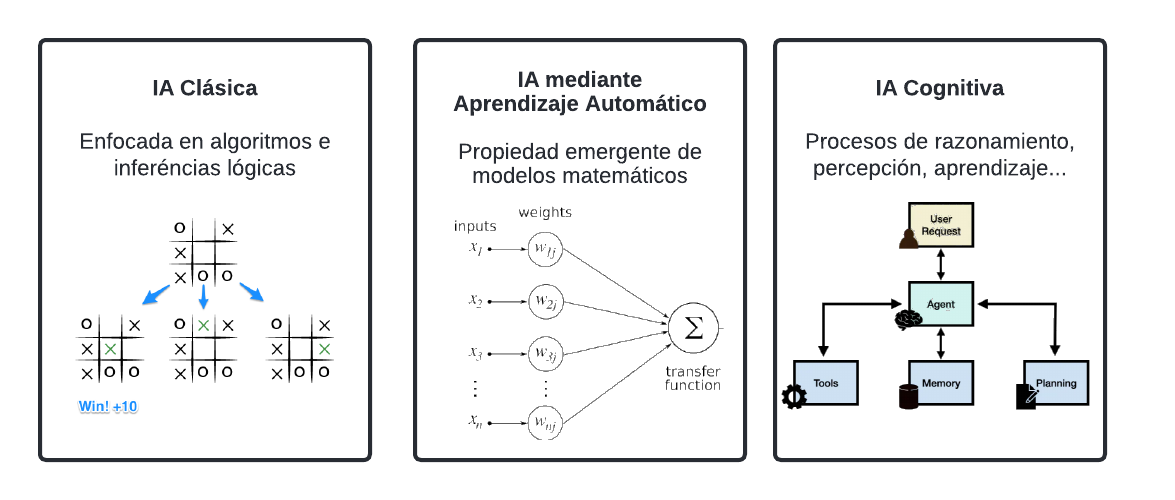
\includegraphics[scale=0.3, trim=0.5cm 0.5cm 0.5cm 0.5cm]{figs/AI-interpretations.png}
    \caption{\small Interpretaciones de Inteligencia Artificial. Elaboración Propia}
    \label{fig:etiqueta}
\end{figure}

\end{itemize}


Durante las décadas posteriores el concepto de inteligencia artificial dio paso a
la investigación de multiples areás sobre lo que se consideraba "inteligente" y como 
estos sectores podian ser automatizados, esto es, convertirlos en elementos artificiales.
Entre las áreas de estudio destacadas encontramos investigaciones sobre la representación
del conocimiento, la inferencia, o la resolución de problemas.

De entre todas estas areas, la resolución de problemas destaca aun a día de hoy
como una de las propiedades mas dificiles de alcanzar. Esto se debe a que
resolver un problema, a diferencia de otras tareas, implica resolver multiples
subtareas que son faciles de para un humano pero a su vez dificilmente
automatizables. Como ejemplo, la tarea de distinguir los comentarios negativos
de los positivos en un foro de internet, resulta trivial de forma intuitiva, sin
embargo matices sutiles del lenguaje como la ironia, gracia, emoción o
exageración resultan imposibles de determinar en un conjunto de pasos que
ejecuta un algoritmo o maquina.

\begin{figure}[!hbp]
    \centering
    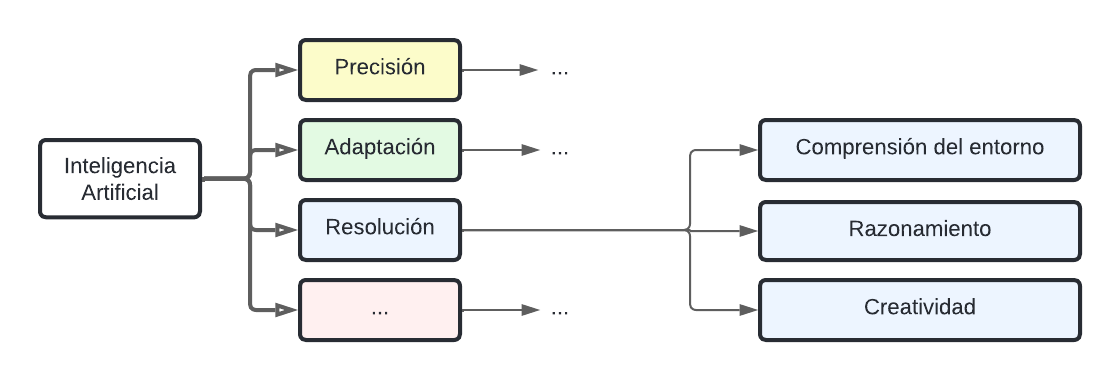
\includegraphics[scale=0.3, trim=0.5cm 0.5cm 0.5cm 0.5cm]{figs/AI-properties.png}
    \caption{\small Requerisitos de la IA. Elaboración Propia}
    \label{fig:etiqueta}
\end{figure}

\section{Fundamentos de la IA Moderna}


\section{Modelos Grandes de Lenguaje}

% Que significa Emerger
% Que es un Agente
% Que es un prompt
% 5 niveles de AGI
\section{Aplicaciones de la IA}

\section{Aprendizaje Automatico vs Inteligencia Artificial}
